% begin module polar-many-representations
\begin{frame}
\begin{columns}[T]
\column{.5\textwidth}
\uncover<1->{
\psset{xunit=2cm, yunit=2cm}
\begin{pspicture}(-0.9, -1.1)(2,0.5)
\tiny
%force a boudning box:
%\psline[linecolor=red!1](-0.1, -0.1)(-0.21,0.2)
%\psline[linecolor=red!1](1.1, 0.6)(1.1,0.61)
\fcFullDotBlue{0}{0}

%Calculator input: plotCurve{}(1/10 \cos{}t, 1/10 \sin{}t, 0, -3/4 \pi)
\parametricplot[arrows=->, linecolor=\fcColorGraph, plotpoints=100]{0} {3.926990817} {t 57.29578 mul cos 0.3000000 mul t 57.29578 mul sin 0.3000000 mul }
\rput[t] (0,-0.1){$O$}
\rput[l](0.3, 0.3){$\theta=\frac{5\pi}{4}$}

\psline{->}(0,0)(2,0)
\psline[linecolor=blue](0,0)(-0.707106781, -0.707106781)
\fcFullDotBlue{-0.707106781}{-0.707106781}
\rput[tl](-0.6, -0.7){$(r,\theta)=\left(1, \frac{5\pi}{4}\right)$}
\end{pspicture}
}
\uncover<2->{
\psset{xunit=2cm, yunit=2cm}
\begin{pspicture}(-0.9, -1.1)(2,0.5)
\tiny
%force a boudning box:
%\psline[linecolor=red!1](-0.1, -0.1)(-0.21,0.2)
\psline[linecolor=red!1](1.1, 0.5)(1.1,0.51)
\fcFullDotBlue{0}{0}

%Calculator input: plotCurve{}(1/10 \cos{}t, 1/10 \sin{}t, 0, -3/4 \pi)
\parametricplot[arrows=->, linecolor=\fcColorGraph, plotpoints=100]{0} {-2.35619} {t 57.29578 mul cos 0.3000000 mul t 57.29578 mul sin 0.3000000 mul }
\rput[t] (0,-0.1){$O$}
\rput[l](0.3, -0.2){$\theta=-\frac{3\pi}{4}$}

\psline{->}(0,0)(2,0)
\psline[linecolor=blue](0,0)(-0.707106781, -0.707106781)
\fcFullDotBlue{-0.707106781}{-0.707106781}
\rput[tl](-0.6, -0.7){$(r,\theta)=\left(1, -\frac{3\pi}{4}\right)$}
\end{pspicture}
}

%\ \uncover<1->{%
%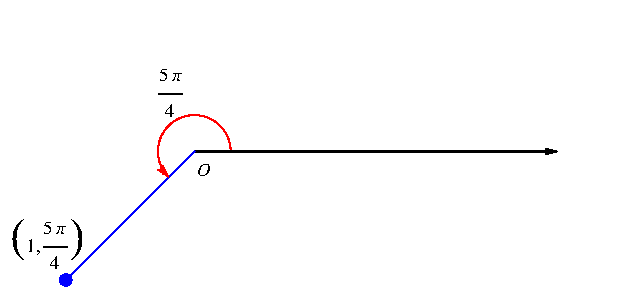
\includegraphics[height=3cm]{polar-curves/pictures/11-03-ex1a.pdf}%
%}%

%\ \uncover<2->{%
%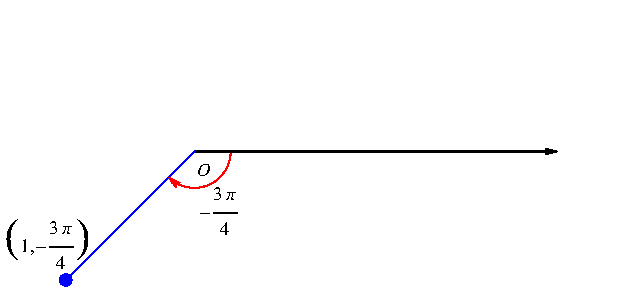
\includegraphics[height=3cm]{polar-curves/pictures/11-03-ex1b.pdf}%
%}%
\column{.5\textwidth}
\uncover<3->{
\psset{xunit=2cm, yunit=2cm}
\begin{pspicture}(-0.9, -1.1)(2,0.5)
\tiny
%force a boudning box:
%\psline[linecolor=red!1](-0.1, -0.1)(-0.21,0.2)
%\psline[linecolor=red!1](1.1, 0.6)(1.1,0.61)
\fcFullDotBlue{0}{0}

%Calculator input: plotCurve{}(1/50 t \cos{}t+3/20 \cos{}t, 1/50 t \sin{}t+3/20 \sin{}t, 0, 13/4 \pi)
\parametricplot[arrows=->, linecolor=\fcColorGraph, plotpoints=400] {0} {10.2102} {t 57.29578 mul cos 0.1500000 mul t 57.29578 mul cos t mul 0.0200000 mul add t 57.29578 mul sin 0.1500000 mul t 57.29578 mul sin t mul 0.0200000 mul add }

\rput[t] (0,-0.1){$O$}
\rput[l](0.3, 0.3){$\theta=\frac{13\pi}{4}$}

\psline{->}(0,0)(2,0)
\psline[linecolor=blue](0,0)(-0.707106781, -0.707106781)
\fcFullDotBlue{-0.707106781}{-0.707106781}
\rput[tl](-0.6, -0.7){$(r,\theta)=\left(1, \frac{13\pi}{4}\right)$}
\end{pspicture}
}

\uncover<4->{
\psset{xunit=2cm, yunit=2cm}
\begin{pspicture}(-0.9, -1.1)(2,0.5)
\tiny
%force a boudning box:
%\psline[linecolor=red!1](-0.1, -0.1)(-0.21,0.2)
\psline[linecolor=red!1](1.1, 0.5)(1.1,0.51)
\fcFullDotBlue{0}{0}

%Calculator input: plotCurve{}(1/10 \cos{}t, 1/10 \sin{}t, 0, -3/4 \pi)
\parametricplot[arrows=->, linecolor=\fcColorGraph, plotpoints=100]{0} {0.785398163} {t 57.29578 mul cos 0.3000000 mul t 57.29578 mul sin 0.3000000 mul }
\rput[t] (0,-0.1){$O$}
\rput[l](0.35, 0.15){$\theta=\frac{\pi}{4}$}

\psline{->}(0,0)(2,0)
\psline[linecolor=blue](0,0)(-0.707106781, -0.707106781)
\fcFullDotBlue{-0.707106781}{-0.707106781}
\psline[linestyle=dashed](0,0)(0.707106781, 0.707106781)
\fcFullDotBlack{0.707106781}{0.707106781}
\rput[tl](-0.6, -0.7){$(r,\theta)=\left(-1, \frac{\pi}{4}\right)$}
\end{pspicture}
}
%\ \uncover<3->{%
%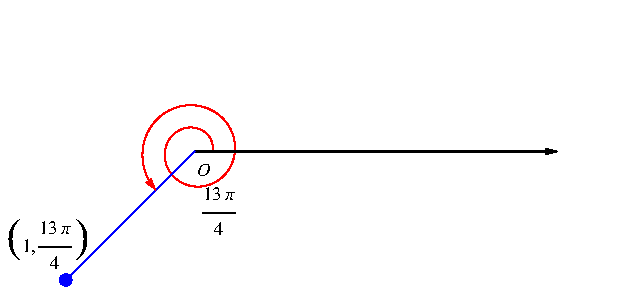
\includegraphics[height=3cm]{polar-curves/pictures/11-03-ex1c.pdf}%
%}%

%\ \uncover<4->{%
%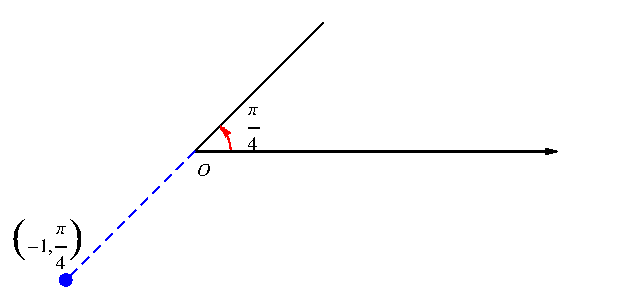
\includegraphics[height=3cm]{polar-curves/pictures/11-03-ex1d.pdf}%
%}%
\end{columns}
\begin{itemize}
\item  There are many ways to represent the same point.
\item<2-| alert@2>  We could use a negative $\theta$.
\item<3-| alert@3>  We could go around more than once.
\item<4-| alert@4>  We could use a negative $r$.
\end{itemize}
\end{frame}
% end module polar-many-representations
